\section{Implementación de OCS-WAF}



\subsection{Arquitectura general}

\begin{frame}
    \frametitle{Detector de anomalías OCS-WAF}

    \begin{center}
        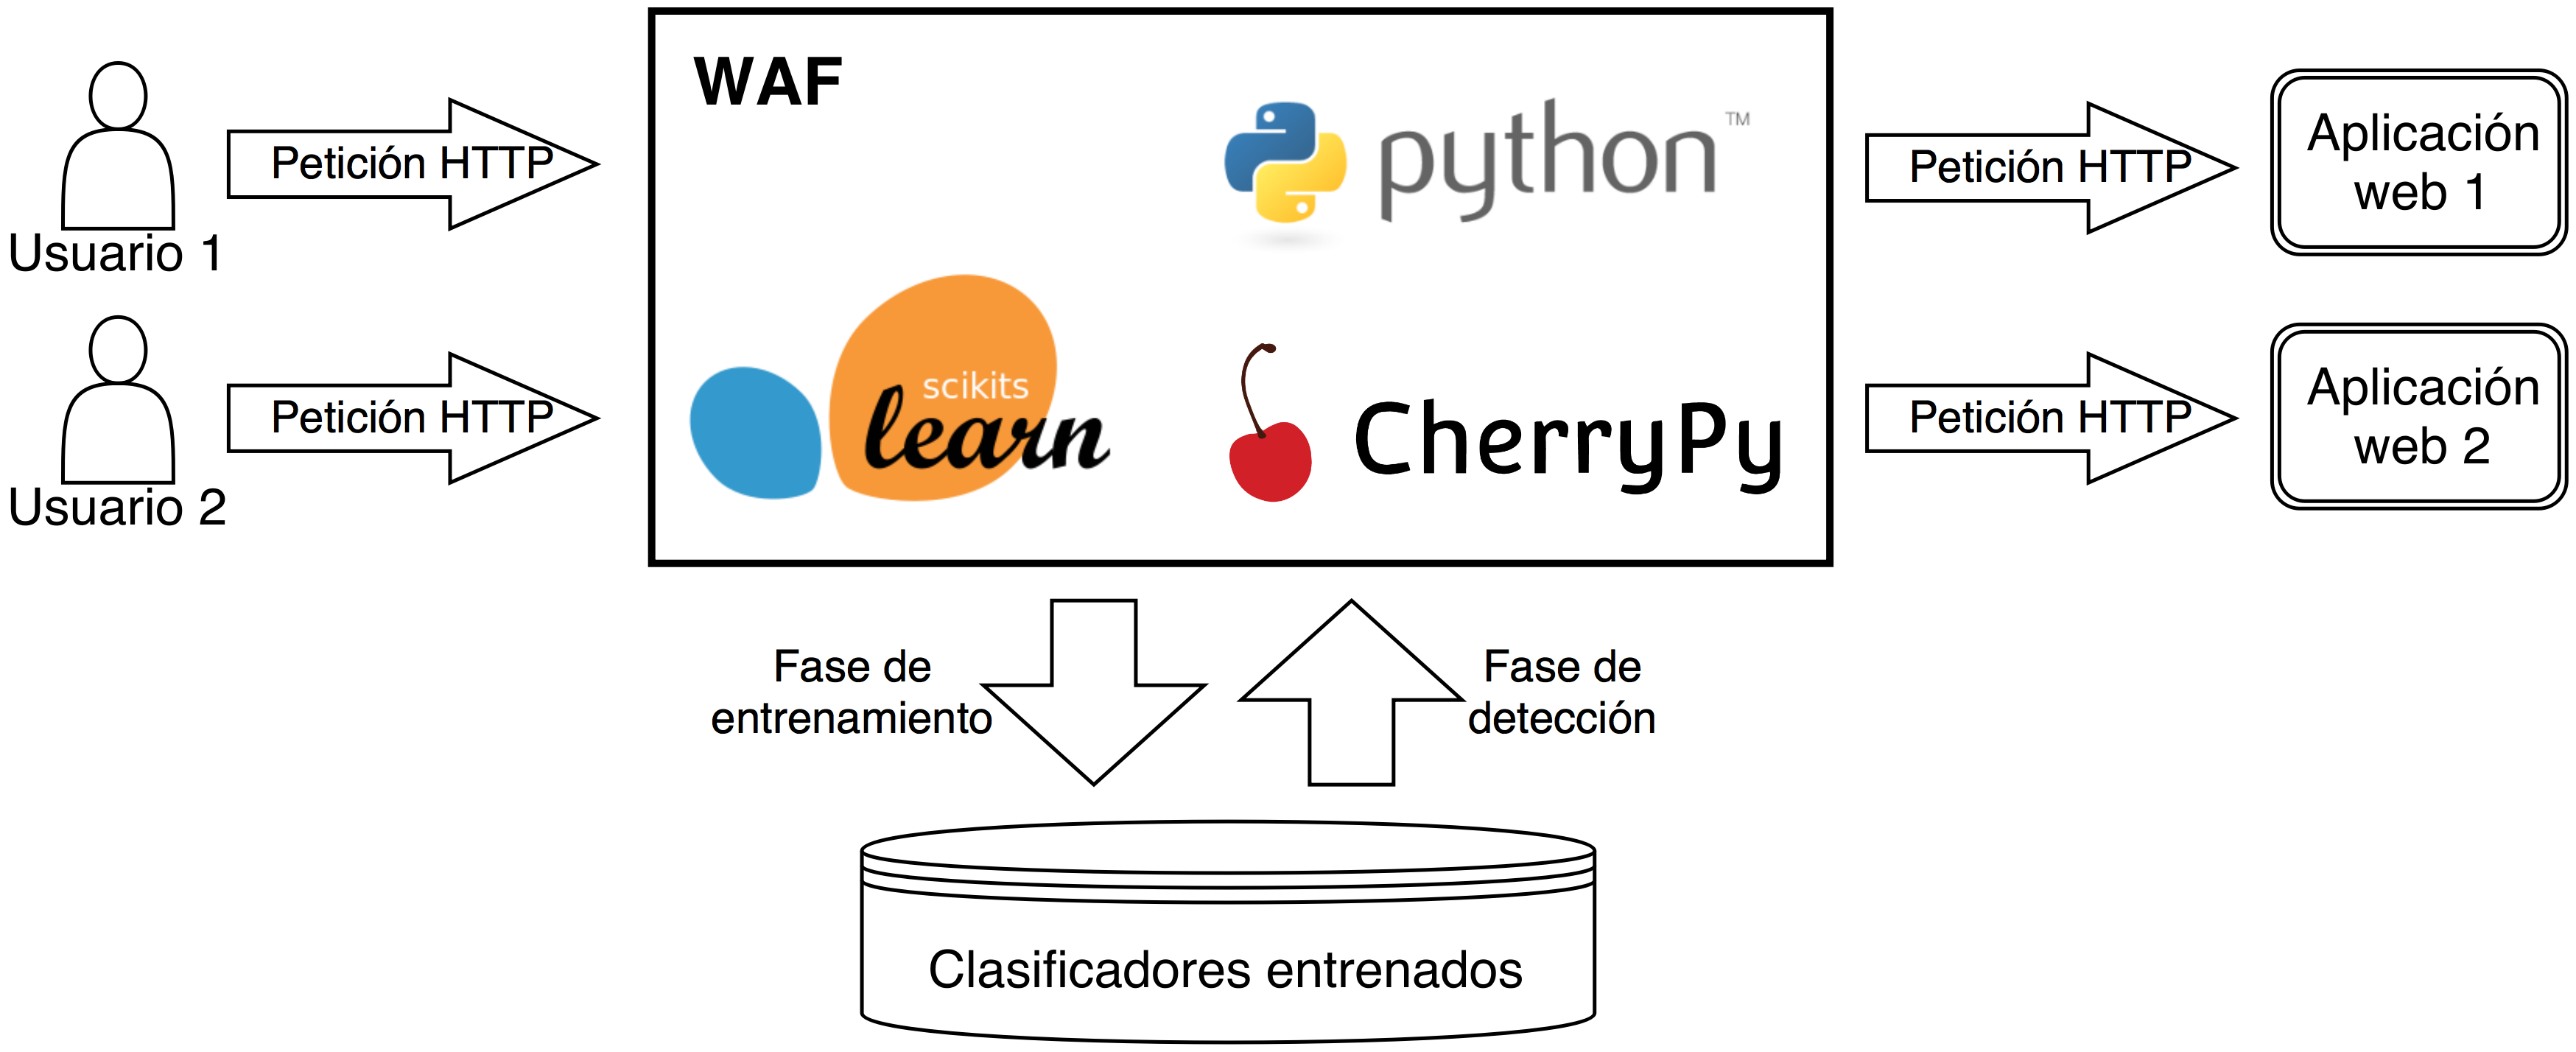
\includegraphics[width=\textwidth]{images/waf-diagram-overview.png}
    \end{center}

    \begin{flushleft}
        \begin{tabular}{l}
            
\includegraphics[height=0.5cm]{images/logo-github.jpg} \\
            \TheRepoUrl \\
        \end{tabular}
    \end{flushleft}
\end{frame}



\subsection{Fase de entrenamiento}

\begin{frame}
    \frametitle{Fase de entrenamiento de OCS-WAF}

    \begin{center}
        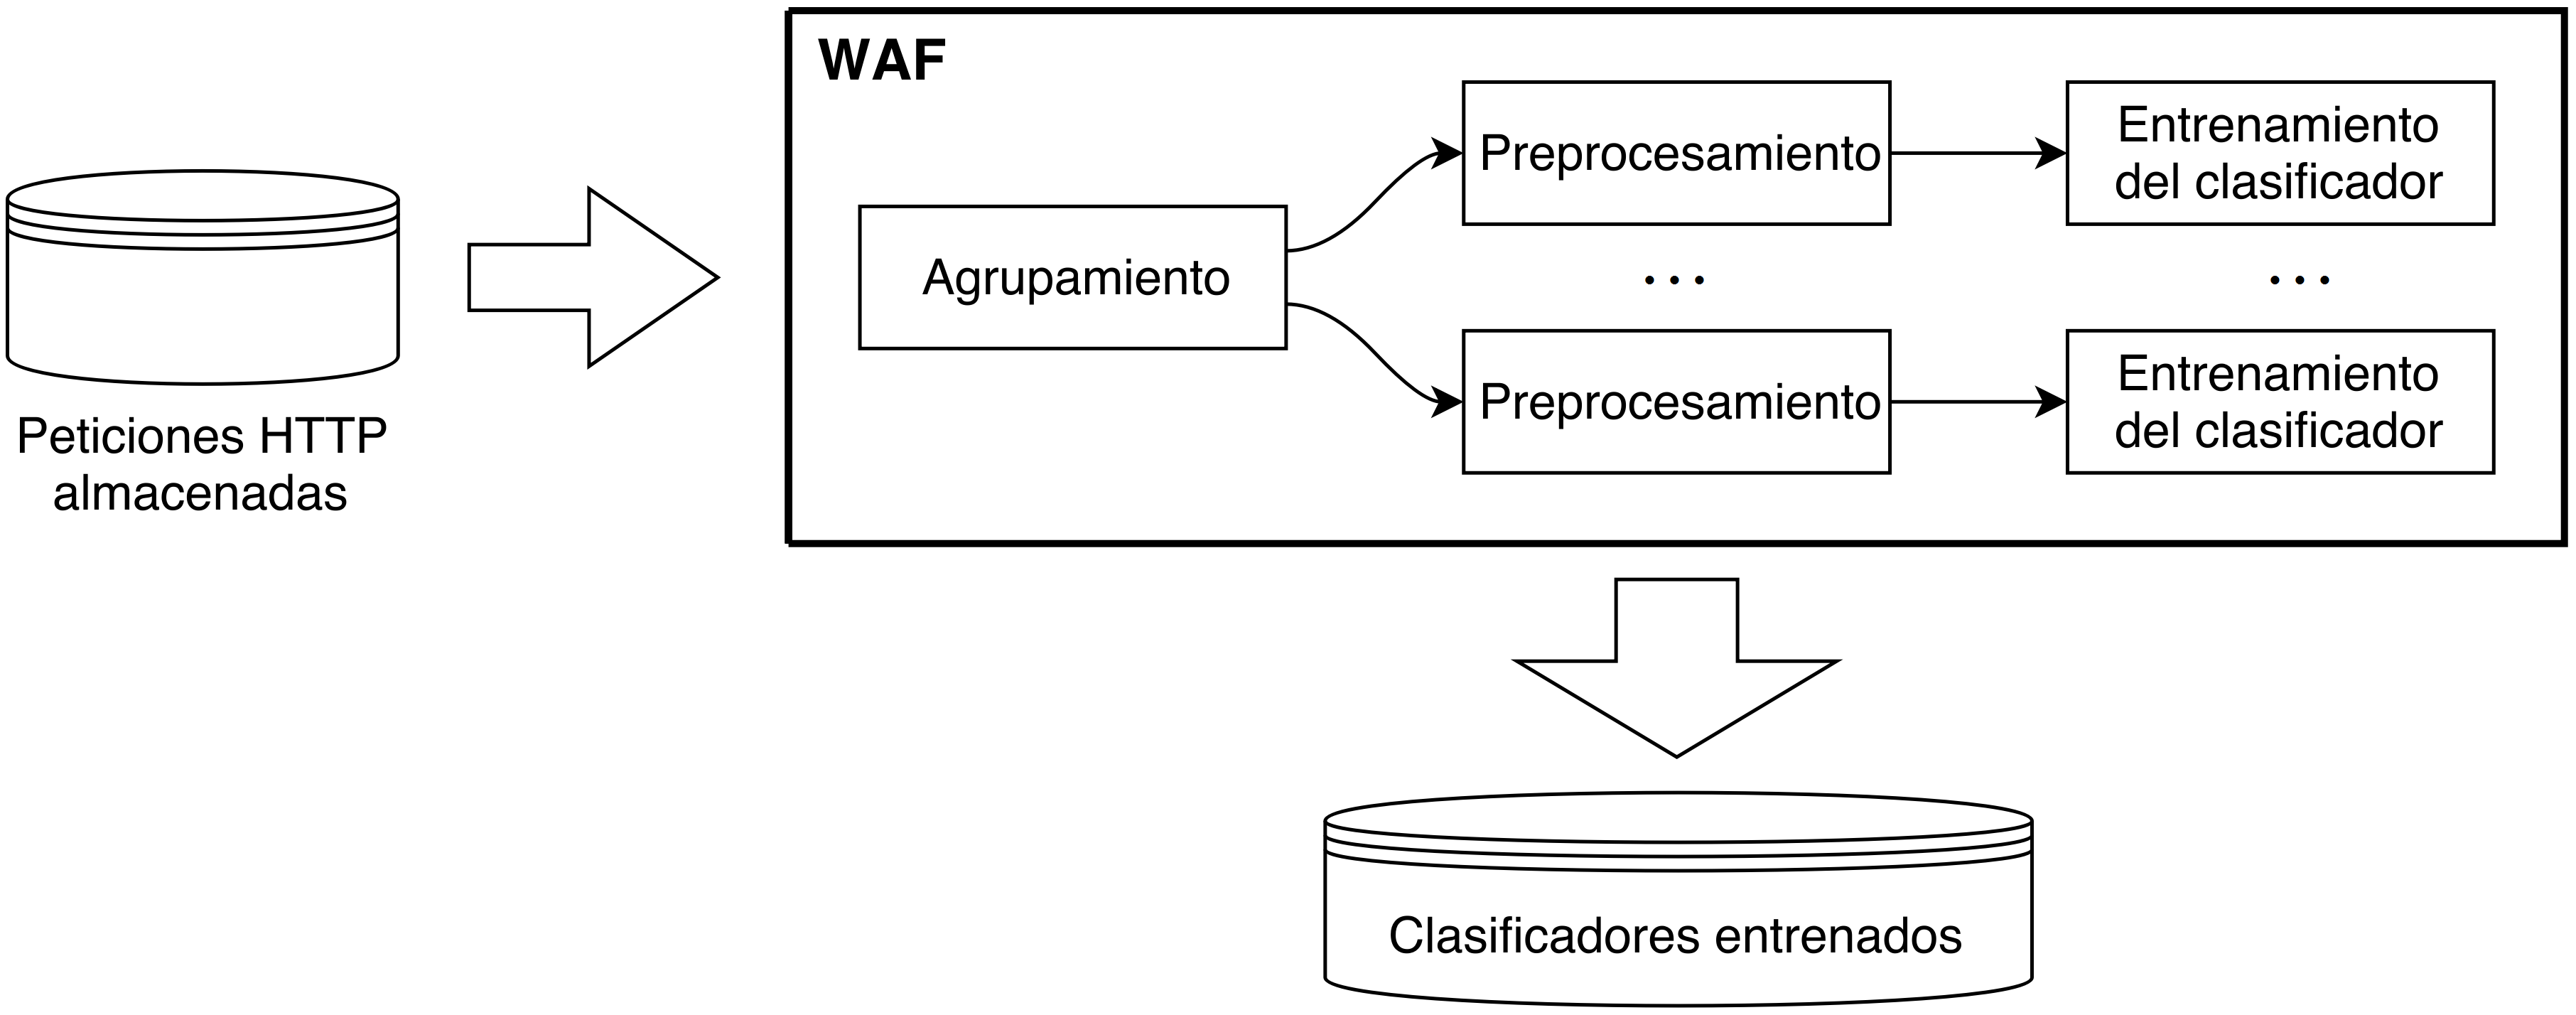
\includegraphics[width=\textwidth]{images/waf-diagram-training.png}
    \end{center}
\end{frame}

\begin{frame}
    \begin{exampleblock}{Estructura de peticiones HTTP}
        \begin{flushleft}
            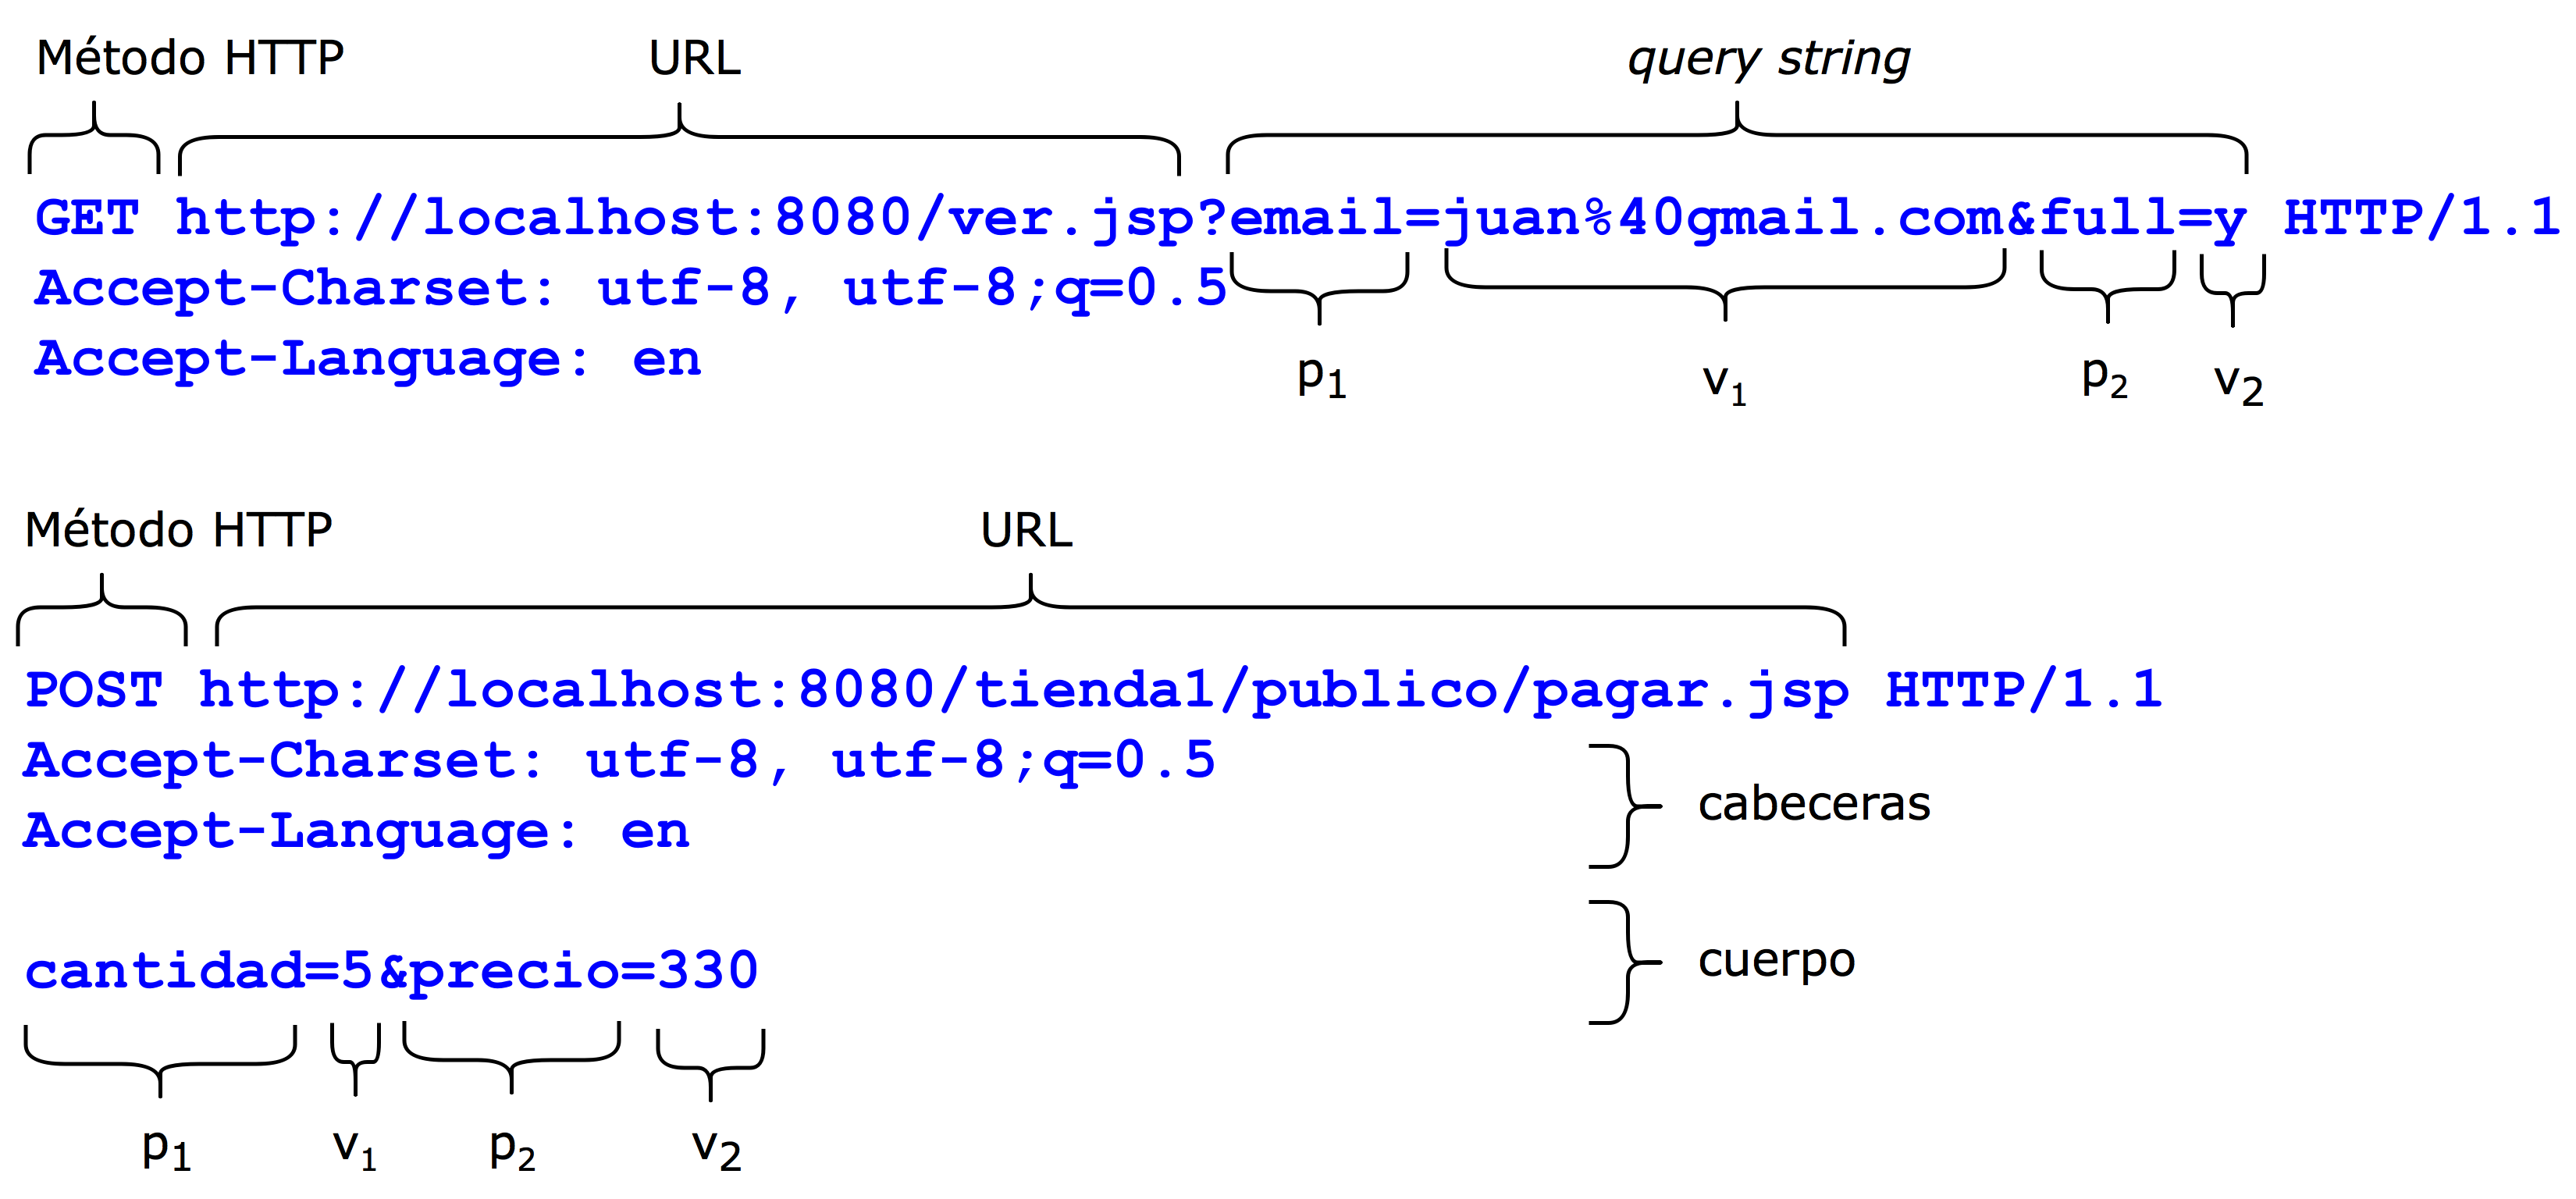
\includegraphics[width=\textwidth]{images/http-request-structure.png}
        \end{flushleft}
    \end{exampleblock}
\end{frame}

\begin{frame}
    \frametitle{1. Paso de agrupamiento}

    \begin{itemize}[<2->]
        \item
        Agrupación por método HTTP y URL

        \begin{flushleft}
            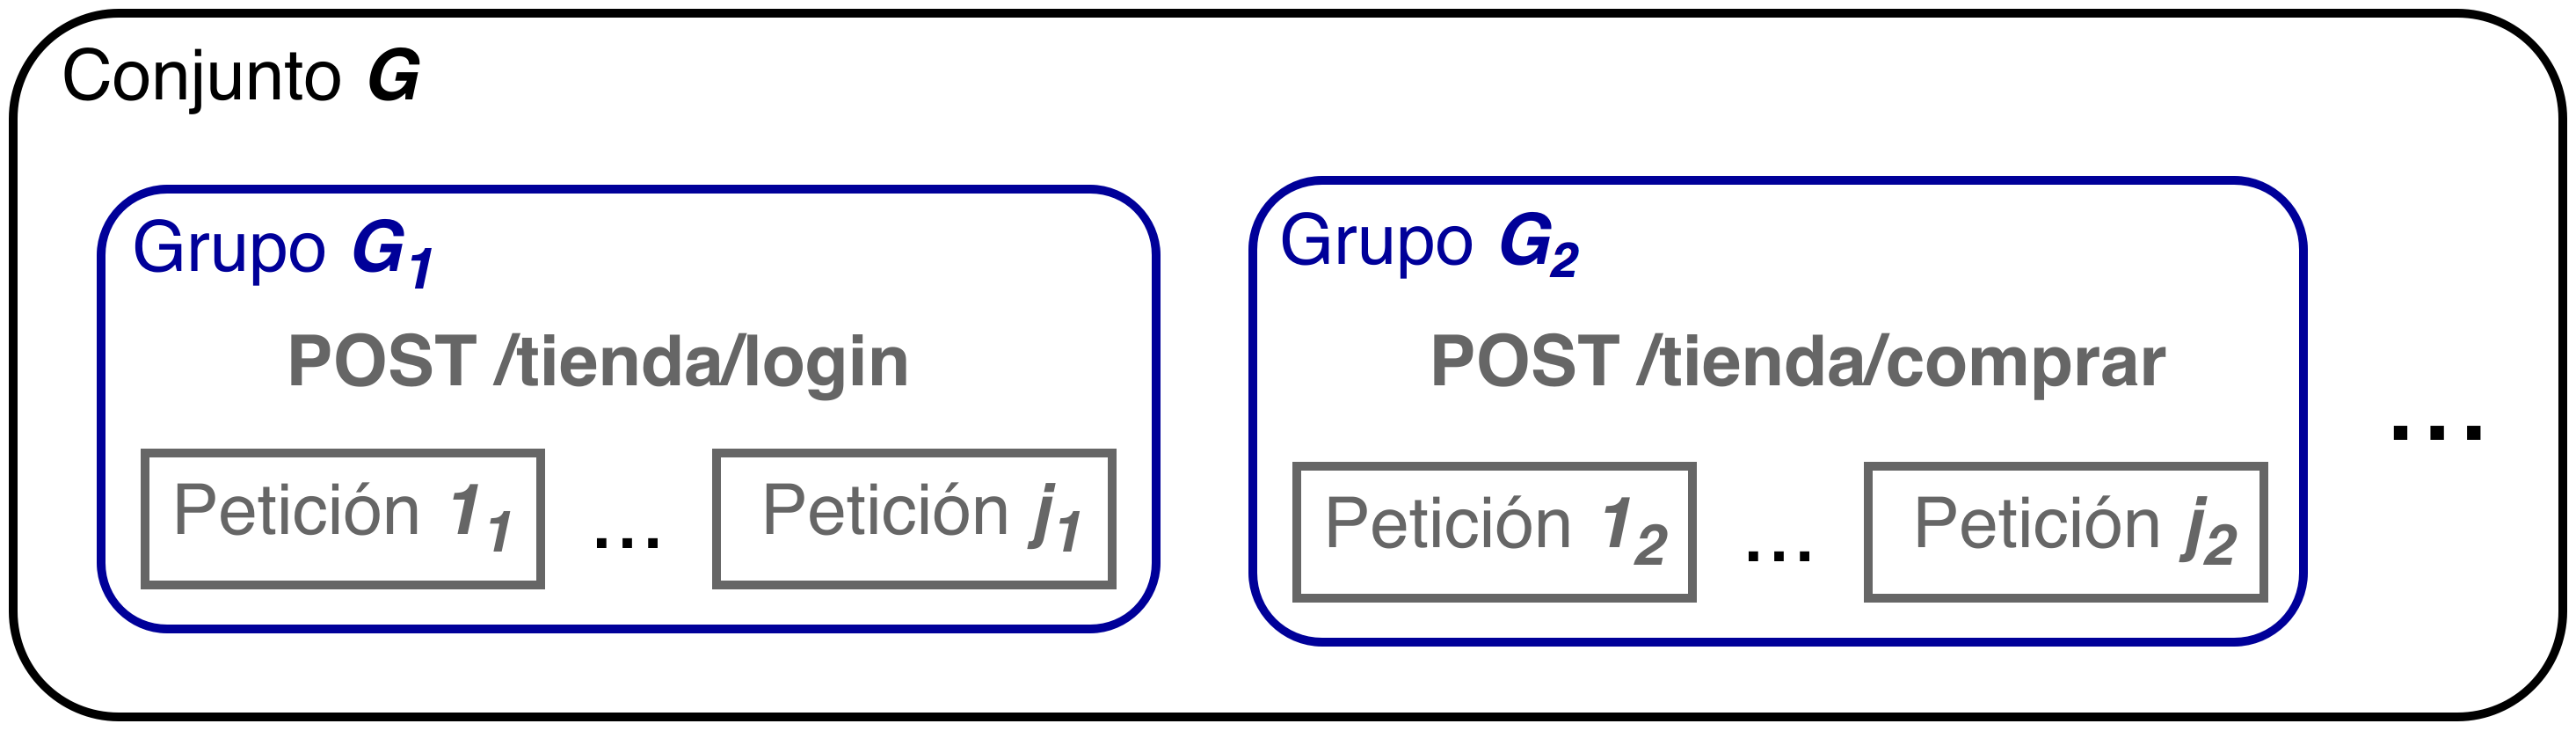
\includegraphics[width=0.9\textwidth]{images/request-groups.png}
        \end{flushleft}

        \item
        Similitud entre peticiones de un mismo grupo $G_{i}$

        \begin{itemize}[<.->]
            \item
            $ \forall i = 1, 2, \dots , \lvert G \rvert $
        \end{itemize}

        \item
        Descripciones más precisas del comportamiento normal dentro de
        cada grupo $G_{i}$
    \end{itemize}
\end{frame}

\begin{frame}
    \frametitle{2. Paso de preprocesamiento}

    \begin{itemize}[<+(1)->]
        \item
        Represetación de características de las peticiones mediante
        vectores numéricos de \textit{features}

        \begin{itemize}[<.->]
            \item
            Petición HTTP $ \quad \rightarrow \quad \vec{f} \in \mathbb{R}^{n} $

            \item
            dimensiones distintas para cada grupo $G_{i}$
        \end{itemize}

        \item
        Características analizadas por OCS-WAF:

        \begin{itemize}[<.->]
            \item
            Distribución de caracteres

            \item
            Entropía

            \item
            Cantidad de caracteres
        \end{itemize}
    \end{itemize}
\end{frame}

\begin{frame}[t]
    \frametitle{2. Paso de preprocesamiento}

    \begin{itemize}
        \item
        Distribución de caracteres

        \begin{itemize}
            \item
            Aporte de Kruegel y Vigna\footnote{
                Kruegel and Vigna (2003) \textit{Anomaly detection of
                web-based attacks}.}

            \item
            Distribución de frecuencias relativas de caracteres

            \item
            Suma de frecuencias relativas en cinco intervalos
        \end{itemize}
    \end{itemize}

    \only<2-3>{
        \begin{center}
            \begin{tikzpicture}
                \node (img1) {
                    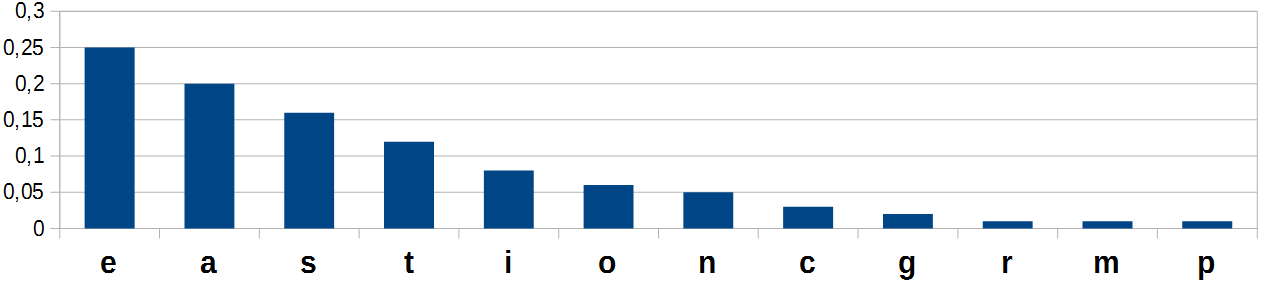
\includegraphics[width=\textwidth]{images/char-distr-blue1.png}
                };
                \node (img2) at (img1.south) [yshift=-0.1cm] {
                    
\includegraphics[width=\textwidth]{images/char-distr-intervals.png}
                };
                \node (img3) at (img1.north) [xshift=3.3cm,yshift=-0.8cm] {
                    \uncover<3->{
                        \frame{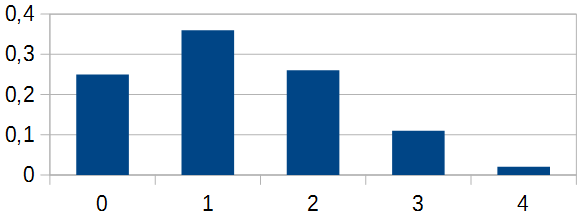
\includegraphics[width=0.4\textwidth]{images/char-distr-blue2.png}}
                    }
                };
            \end{tikzpicture}
        \end{center}
    }
    \only<4->{
        \begin{center}
            \begin{tikzpicture}
                \node (img1) {
                    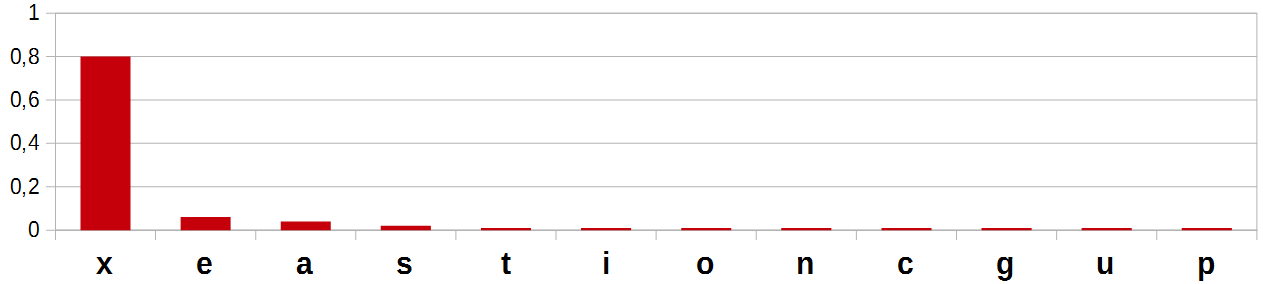
\includegraphics[width=\textwidth]{images/char-distr-red1.png}
                };
                \node (img2) at (img1.south) [yshift=-0.1cm] {
                    
\includegraphics[width=\textwidth]{images/char-distr-intervals.png}
                };
                \node (img3) at (img1.north) [xshift=3.3cm,yshift=-0.8cm] {
                    \uncover<5->{
                        \frame{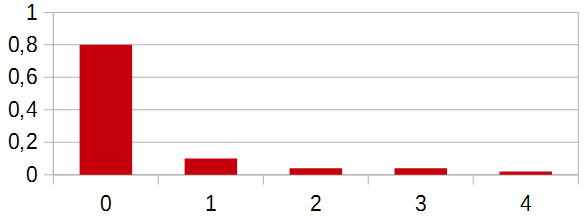
\includegraphics[width=0.4\textwidth]{images/char-distr-red2.png}}
                    }
                };
            \end{tikzpicture}
        \end{center}
    }
\end{frame}

\begin{frame}[t]
    \frametitle{2. Paso de preprocesamiento}

    \begin{itemize}
        \item
        Entropía (Teoría de la información)

        \begin{itemize}
            \item
            Relación entre longitud del valor y cantidad de caracteres
            distintos

            \item
            Aporte de Nguyen et. al.\footnote{
                Nguyen et. al. (2011) \textit{Application of the generic
                feature selection measure in detection of web attacks}.}

            \item
            Fórmula propuesta por Claude Shannon\footnote{
                Shannon (1948) \textit{A Mathematical Theory of Communication}.}
        \end{itemize}
    \end{itemize}

    \only<1>{
        \begin{columns}
            \column{0.6\textwidth}
            $$
            H(x) =
            - \sum_{i=1}^{\lvert c \rvert}
            \left(
                \frac{c_{i}}{\lvert x \rvert} \times \log_{2} \frac{c_{i}}{\lvert x \rvert}
            \right)
            $$

            \column{0.4\textwidth}
            \begin{block}{\small Ejemplo}
                \small
                $x = \text{aabbc}$

                $\lvert x \rvert = 5$

                $\lvert c \rvert = 3$

                $c_{1} = 2 \quad \rightarrow \quad \text{a}$

                $c_{2} = 2 \quad \rightarrow \quad \text{b}$

                $c_{3} = 1 \quad \rightarrow \quad \text{c}$
            \end{block}
        \end{columns}
    }
    \only<2->{
        \begin{columns}
            \column{0.4\textwidth}
            \begin{block}{\small Ejemplo: petición normal}
                \begin{itemize}
                    \item
                    \small $H(x) = \num{5.092}$
                \end{itemize}
            \end{block}

            \column{0.6\textwidth}
            \begin{block}{\small Ejemplo: petición con \textit{buffer overflow}}
                \begin{itemize}
                    \item
                    \small $H(x) = 0.901$
                \end{itemize}
            \end{block}
        \end{columns}
    }
\end{frame}

\begin{frame}[t]
    \frametitle{2. Paso de preprocesamiento}

    \begin{itemize}
        \item
        Cantidad de caracteres

        \begin{itemize}
            \item
            Aporte de Kruegel y Vigna\footnote{
                Kruegel and Vigna (2003) \textit{Anomaly detection of
                web-based attacks}.},
            y Nguyen et. al.\footnote{
                Nguyen et. al. (2011) \textit{Application of the generic
                feature selection measure in detection of web attacks}.}

            \item
            Conjuntos de caracteres

            \begin{enumerate}
                \item Todos
                \item Dígitos
                \item Letras
                \item Otros caracteres
            \end{enumerate}
        \end{itemize}
    \end{itemize}

    \uncover<2->{
        \begin{columns}
            \column{0.4\textwidth}
            \begin{block}{\small Ejemplo: petición normal}
                \vspace{-0.3cm}
                \begin{flushleft}
                    \small
                    \begin{tabular}{lcr}
                        Todos   & = & \num{100} \\
                        Dígitos & = &   \num{9} \\
                        Letras  & = &  \num{74} \\
                        Otros   & = &  \num{17} \\
                    \end{tabular}
                \end{flushleft}
            \end{block}

            \column{0.6\textwidth}
            \begin{block}{\small Ejemplo: petición con \textit{code injection}}
                \vspace{-0.3cm}
                \begin{flushleft}
                    \small
                    \begin{tabular}{lcr}
                        Todos   & = &       \num{132}  \\
                        Dígitos & = & \alert{\num{21}} \\
                        Letras  & = &        \num{78}  \\
                        Otros   & = & \alert{\num{33}} \\
                    \end{tabular}
                \end{flushleft}
            \end{block}
        \end{columns}
    }
\end{frame}

\begin{frame}
    \frametitle{2. Paso de preprocesamiento}

    \begin{itemize}
        \item
        10 \textit{features} extraídos
    \end{itemize}

    \begin{center}
        \small
        \begin{tabular}{|l|c|c|}
            \hline
            \multicolumn{1}{|c|}{\textit{Features}} & Tipo de dato & Rango de valores \\ \specialrule{1.5pt}{0}{0}
            Dist. de caract. - intervalo 0          & núm. reales  & $[0, 1]$         \\ \hline
            Dist. de caract. - intervalo 1          & núm. reales  & $[0, 1]$         \\ \hline
            Dist. de caract. - intervalo 2          & núm. reales  & $[0, 1]$         \\ \hline
            Dist. de caract. - intervalo 3          & núm. reales  & $[0, 1]$         \\ \hline
            Dist. de caract. - intervalo 4          & núm. reales  & $[0, 1]$         \\ \hline
            Entropía                                & núm. reales  & $[0, \infty)$    \\ \hline
            Longitud o cantidad total               & núm. enteros & $[0, \infty)$    \\ \hline
            Cantidad de dígitos                     & núm. enteros & $[0, \infty)$    \\ \hline
            Cantidad de letras                      & núm. enteros & $[0, \infty)$    \\ \hline
            Cantidad de otros caracteres            & núm. enteros & $[0, \infty)$    \\ \hline
        \end{tabular}
    \end{center}
\end{frame}

\begin{frame}
    \frametitle{2. Paso de preprocesamiento}

    \begin{itemize}[<+->]
        \item
        Análisis de valores de parámetros

        \begin{itemize}[<.->]
            \item
            Obtención de parámetros presentes en peticiones de $G_{i}$

            \begin{itemize}
                \item
                $ Q_{i} \ = \ [ \ \text{"email"} \ , \ \text{"full"} \ ] $

                \item
                $ B_{i} \ = \ [ \ ] $
            \end{itemize}

            \item
            Extracción de \textit{features} de cada valor de los parámetros
        \end{itemize}
    \end{itemize}

    \begin{flushleft}
        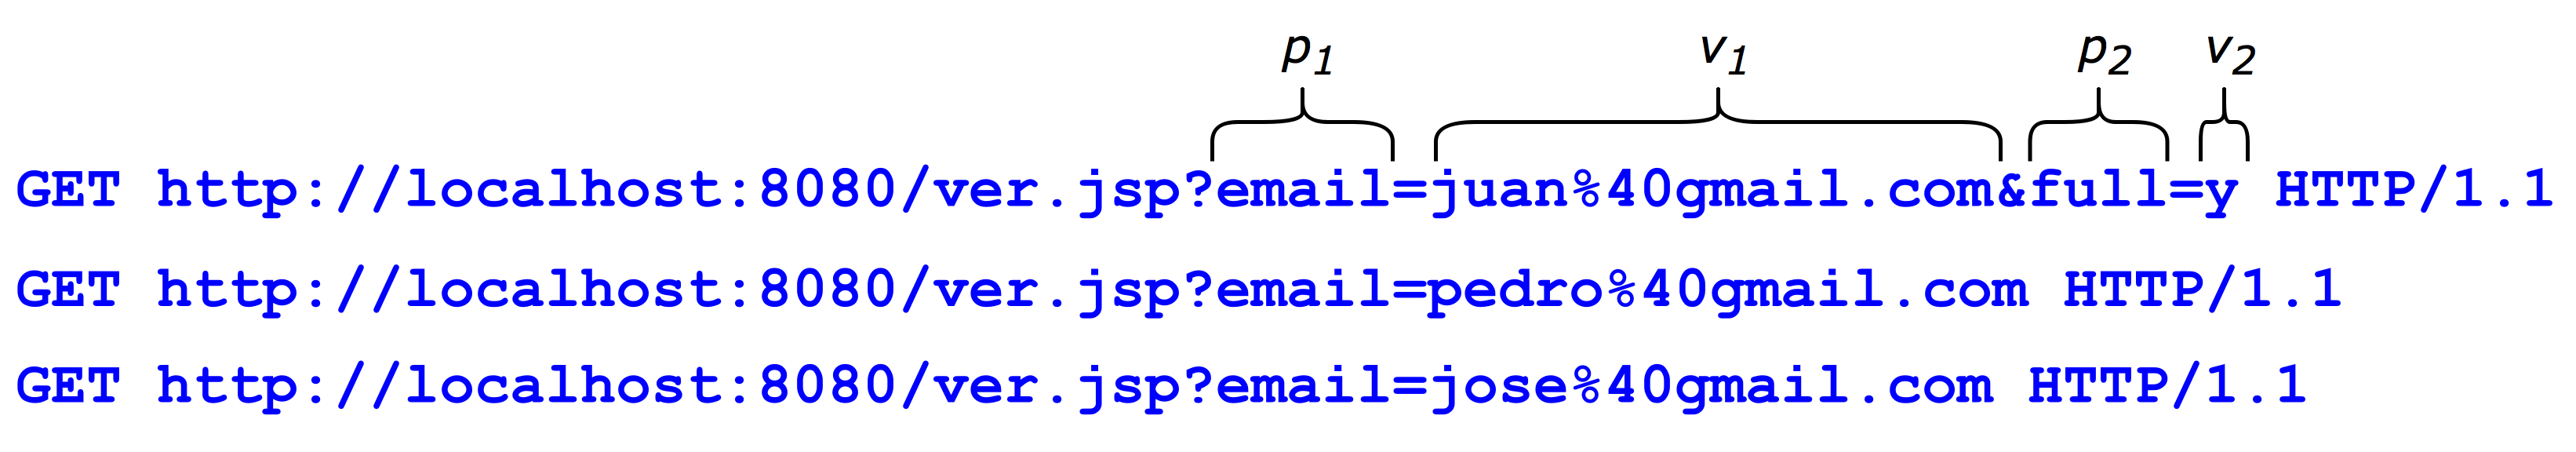
\includegraphics[width=\textwidth]{images/request-examples-1.png}
    \end{flushleft}
\end{frame}

\begin{frame}
    \frametitle{2. Paso de preprocesamiento}

    \begin{itemize}[<+->]
        \item
        Composición del vector de \textit{features}

        \begin{itemize}[<.->]
            \item
            Dimensiones según los parámetros en cada grupo $G_{i}$

            \item
            $ n_{i} = 10 \times \left( 1 + \lvert Q_{i} \rvert + \lvert B_{i} \rvert \right) $
        \end{itemize}
    \end{itemize}

    \begin{center}
        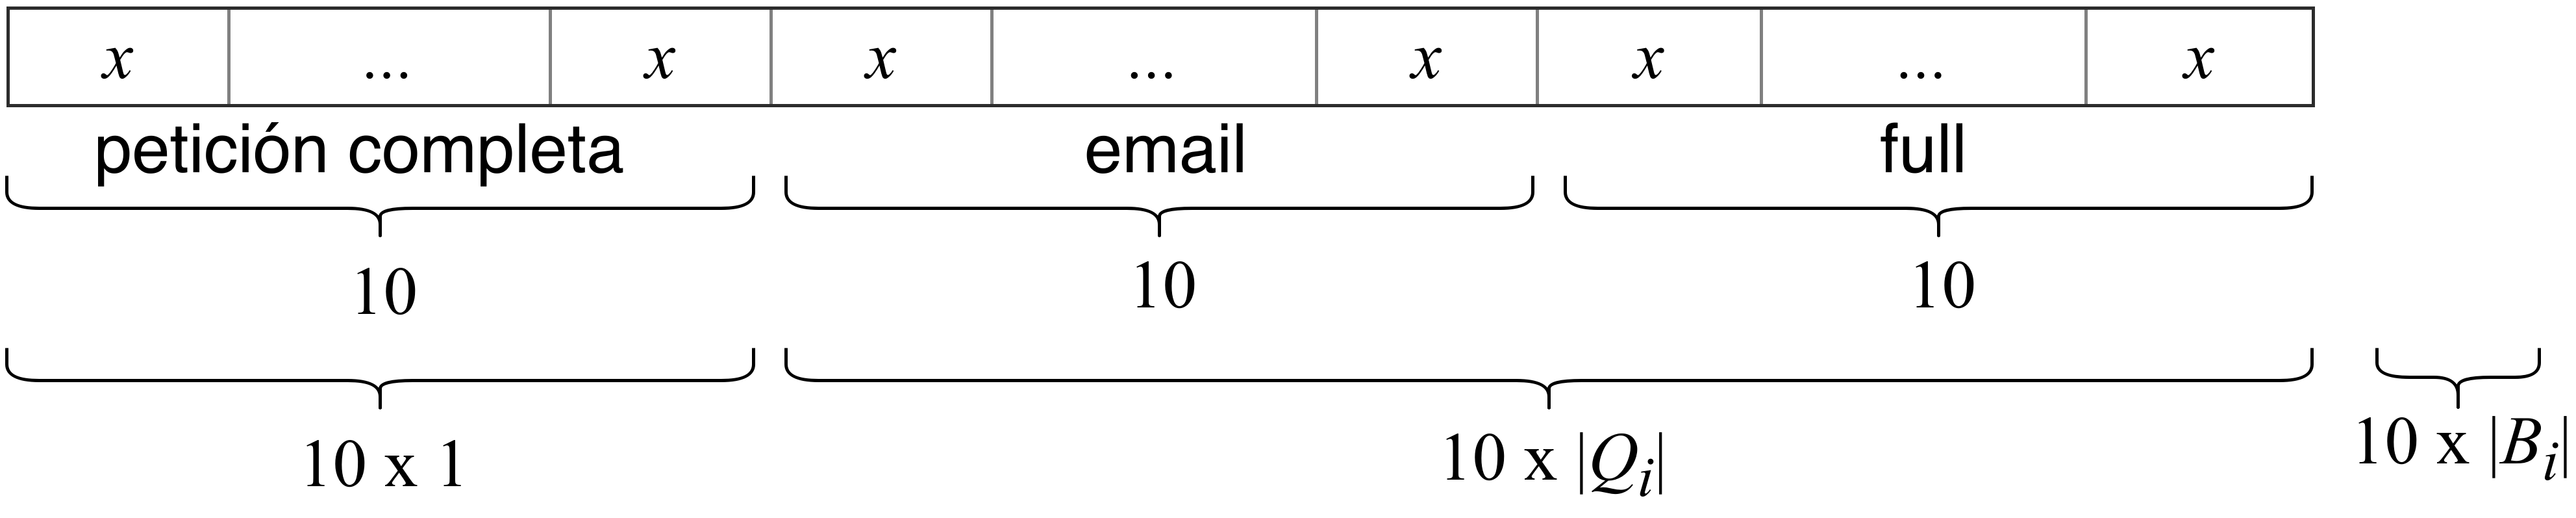
\includegraphics[width=\textwidth]{images/composition-vector.png}
    \end{center}

    \begin{flushleft}
        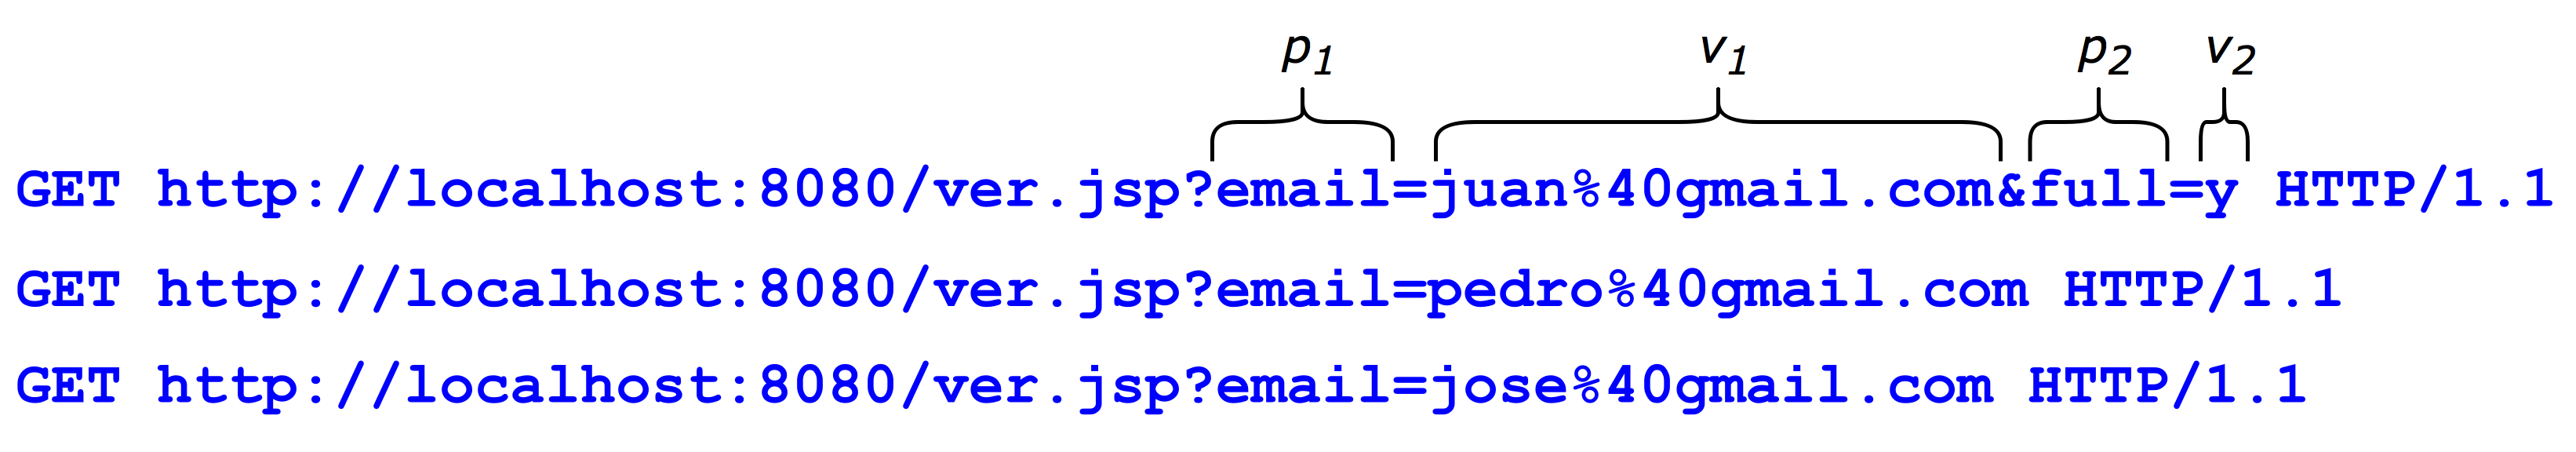
\includegraphics[width=\textwidth]{images/request-examples-1.png}
    \end{flushleft}
\end{frame}

\begin{frame}
    \frametitle{2. Paso de preprocesamiento}

    \begin{itemize}[<+->]
        \item
        Composición de la matriz de vectores de \textit{features}

        \begin{itemize}[<.->]
            \item
            Filas: vectores de peticiones del grupo $G_{i}$

            \item
            Columnas: \textit{features} del grupo $G_{i}$
        \end{itemize}
    \end{itemize}

    \begin{center}
        $$
        M_{i} =
        \begin{bmatrix}
            x_{1,1}                    & x_{1,2}                    & \cdots & x_{1,n_{i}} \\
            x_{2,1}                    & x_{2,2}                    & \cdots & x_{2,n_{i}} \\
            \vdots                     & \vdots                     & \ddots & \vdots      \\
            x_{\lvert G_{i} \rvert, 1} & x_{\lvert G_{i} \rvert, 2} & \cdots & x_{\lvert G_{i} \rvert, n_{i}}
        \end{bmatrix}
        $$
    \end{center}
\end{frame}

\begin{frame}
    \frametitle{2. Paso de preprocesamiento}

    \begin{itemize}
        \item
        Escalamiento de \textit{features} (normalización)

        \begin{itemize}
            \item
            Problema:

            \begin{itemize}
                \item
                Distintas importancias de \textit{features} debido a
                rangos diferentes
            \end{itemize}

            \item<2->
            Finalidad del escalamiento estándar\footnote{Rieck (2009) Machine
                Learning for Application-Layer Intrusion Detection}:

            \begin{itemize}[<2->]
                \item
                Promedio cercano a 0 y una varianza cercana a 1 en cada
                \textit{feature} (cada columna de $M_{i}$)
            \end{itemize}
        \end{itemize}
    \end{itemize}

    \uncover<2->{
        \begin{flushleft}
            $$
            x_{\text{\tiny nuevo}}
            \ = \
            \frac
                {x_{\text{\tiny actual}} - \mu_{\text{\tiny de la columna}}}
                {\sigma_{\text{\tiny de la columna}}}
            $$
        \end{flushleft}
    }
\end{frame}

\begin{frame}
    \begin{exampleblock}{\textit{Support Vector Machine} (SVM)}
        \begin{itemize}
            \item
            Clasificadores binarios de aprendizaje supervisado

            \item
            Separación de clases mediante un hiperplano
        \end{itemize}
    \end{exampleblock}

    \begin{columns}
        \column{0.5\textwidth}
        \uncover<2->{
            \begin{exampleblock}{One-Class SVM}
                \begin{itemize}
                    \item
                    Versión modificada para problemas OCC

                    \item
                    Separación de única clase del origen% mediante hiperplano

                    \item<3->
                    Transformación a otros espacios

                    \begin{itemize}[<.->]
                        \item
                        \textit{Radial Basis Function} (RBF) kernel
                    \end{itemize}
                \end{itemize}
            \end{exampleblock}
        }

        \column{0.5\textwidth}
        \begin{center}
            \only<1>{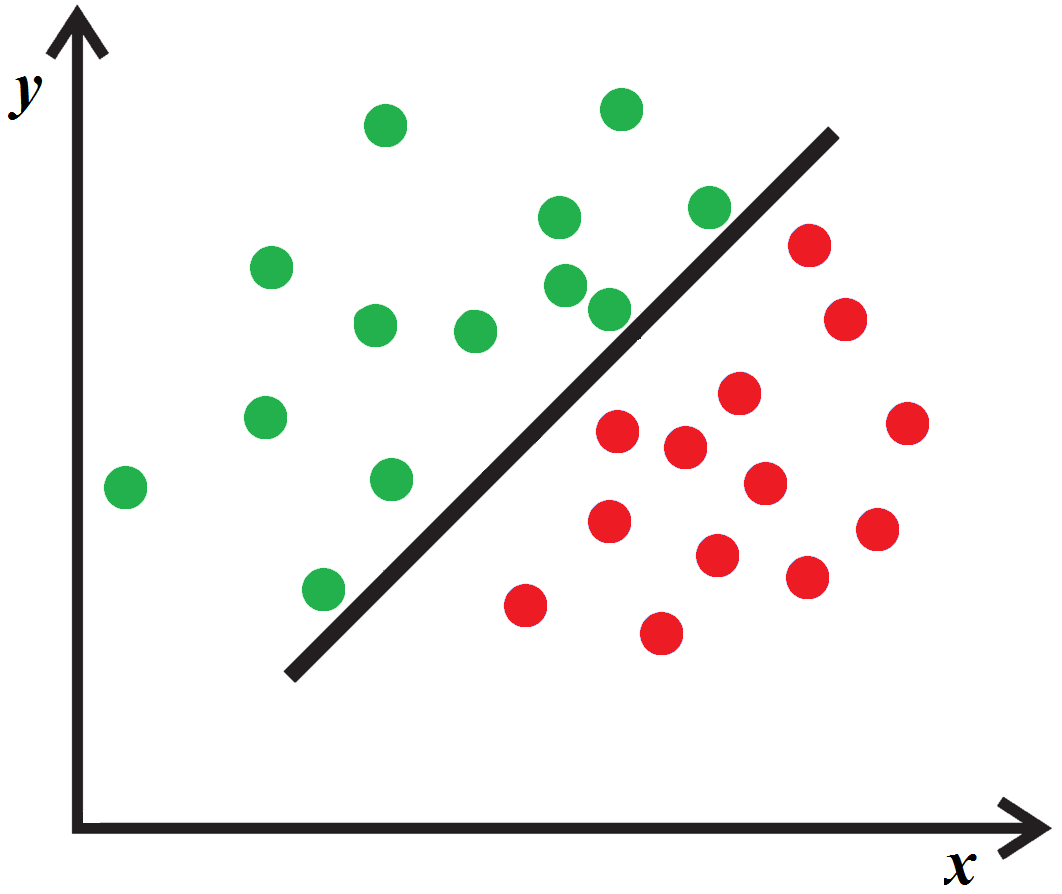
\includegraphics[width=\textwidth]{images/svm-example-1.png}}
            \only<2>{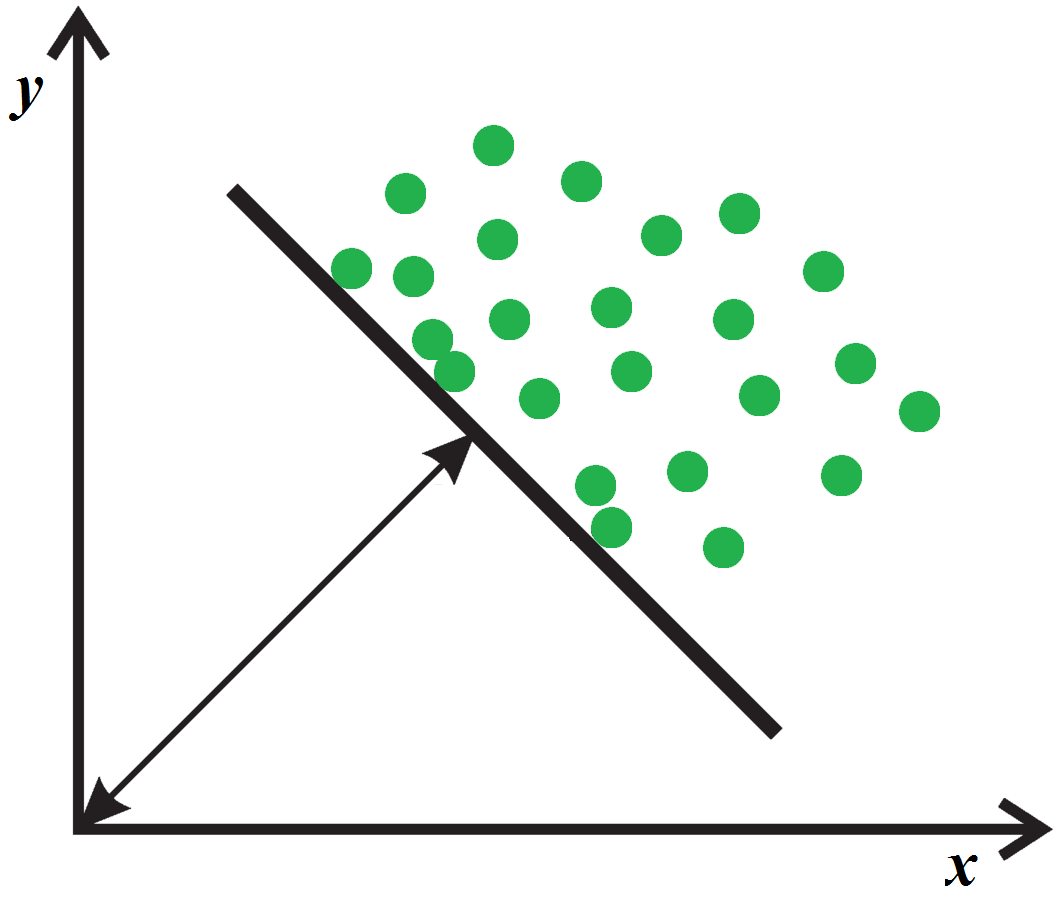
\includegraphics[width=\textwidth]{images/ocsvm-example-1.png}}
            \only<3->{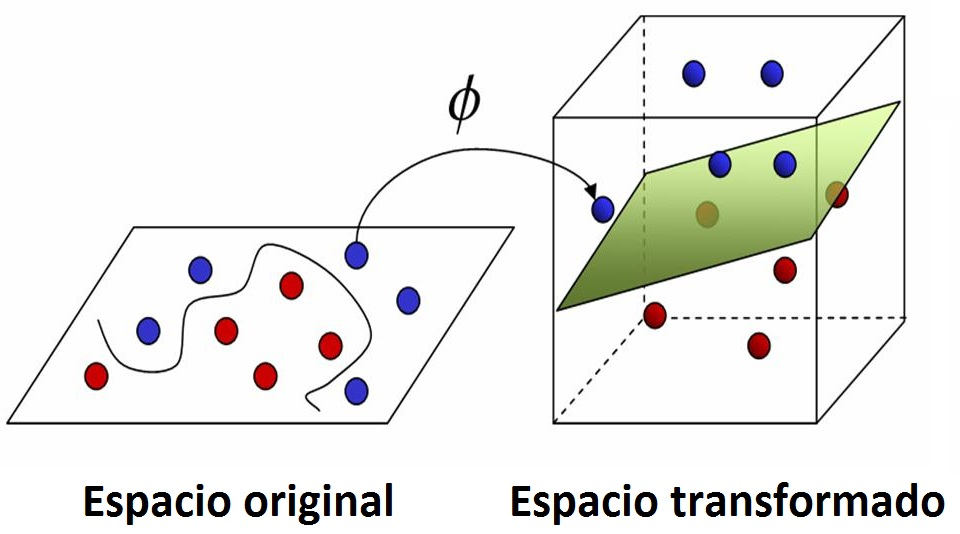
\includegraphics[width=\textwidth]{images/svm-transformed-space.jpg}}
        \end{center}
    \end{columns}
\end{frame}

\begin{frame}
    \frametitle{3. Paso de entrenamiento de clasificadores}

    \begin{columns}
        \column{0.5\textwidth}
        \begin{itemize}[<2->]
            \item
            Un One-Class SVM por cada grupo $G_{i}$

            \item
            Entrenamiento con los vectores de \textit{features}
            construidos

            \begin{itemize}[<.->]
                \item
                Matrices $M_{i}$
            \end{itemize}

            \item
            Gran cantidad de \textit{features}

            \item
            Almacenamiento persistente de clasificadores entrenados
        \end{itemize}

        \column{0.5\textwidth}
        \begin{center}
            \uncover<2->{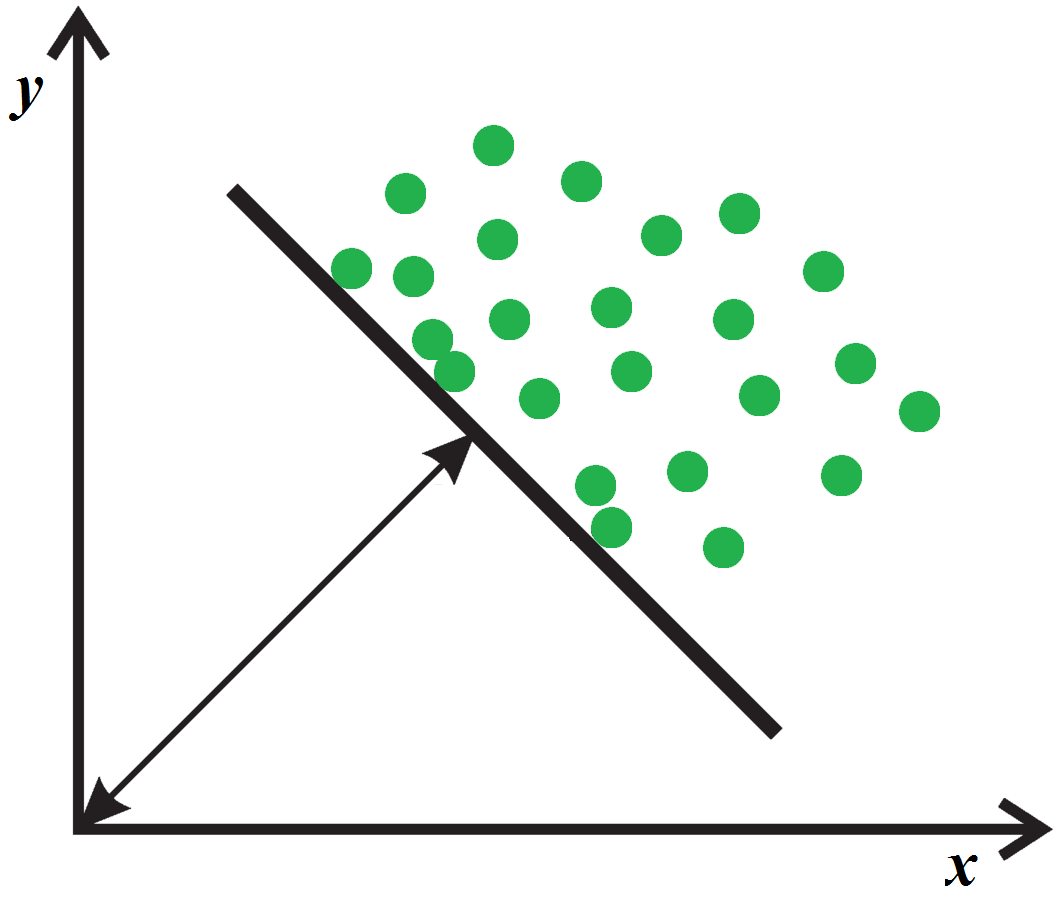
\includegraphics[width=\textwidth]{images/ocsvm-example-1.png}}
        \end{center}
    \end{columns}
\end{frame}



\subsection{Fase de detección}

\begin{frame}
    \frametitle{Fase de detección}

    \begin{center}
        \hspace*{-0.75cm}
        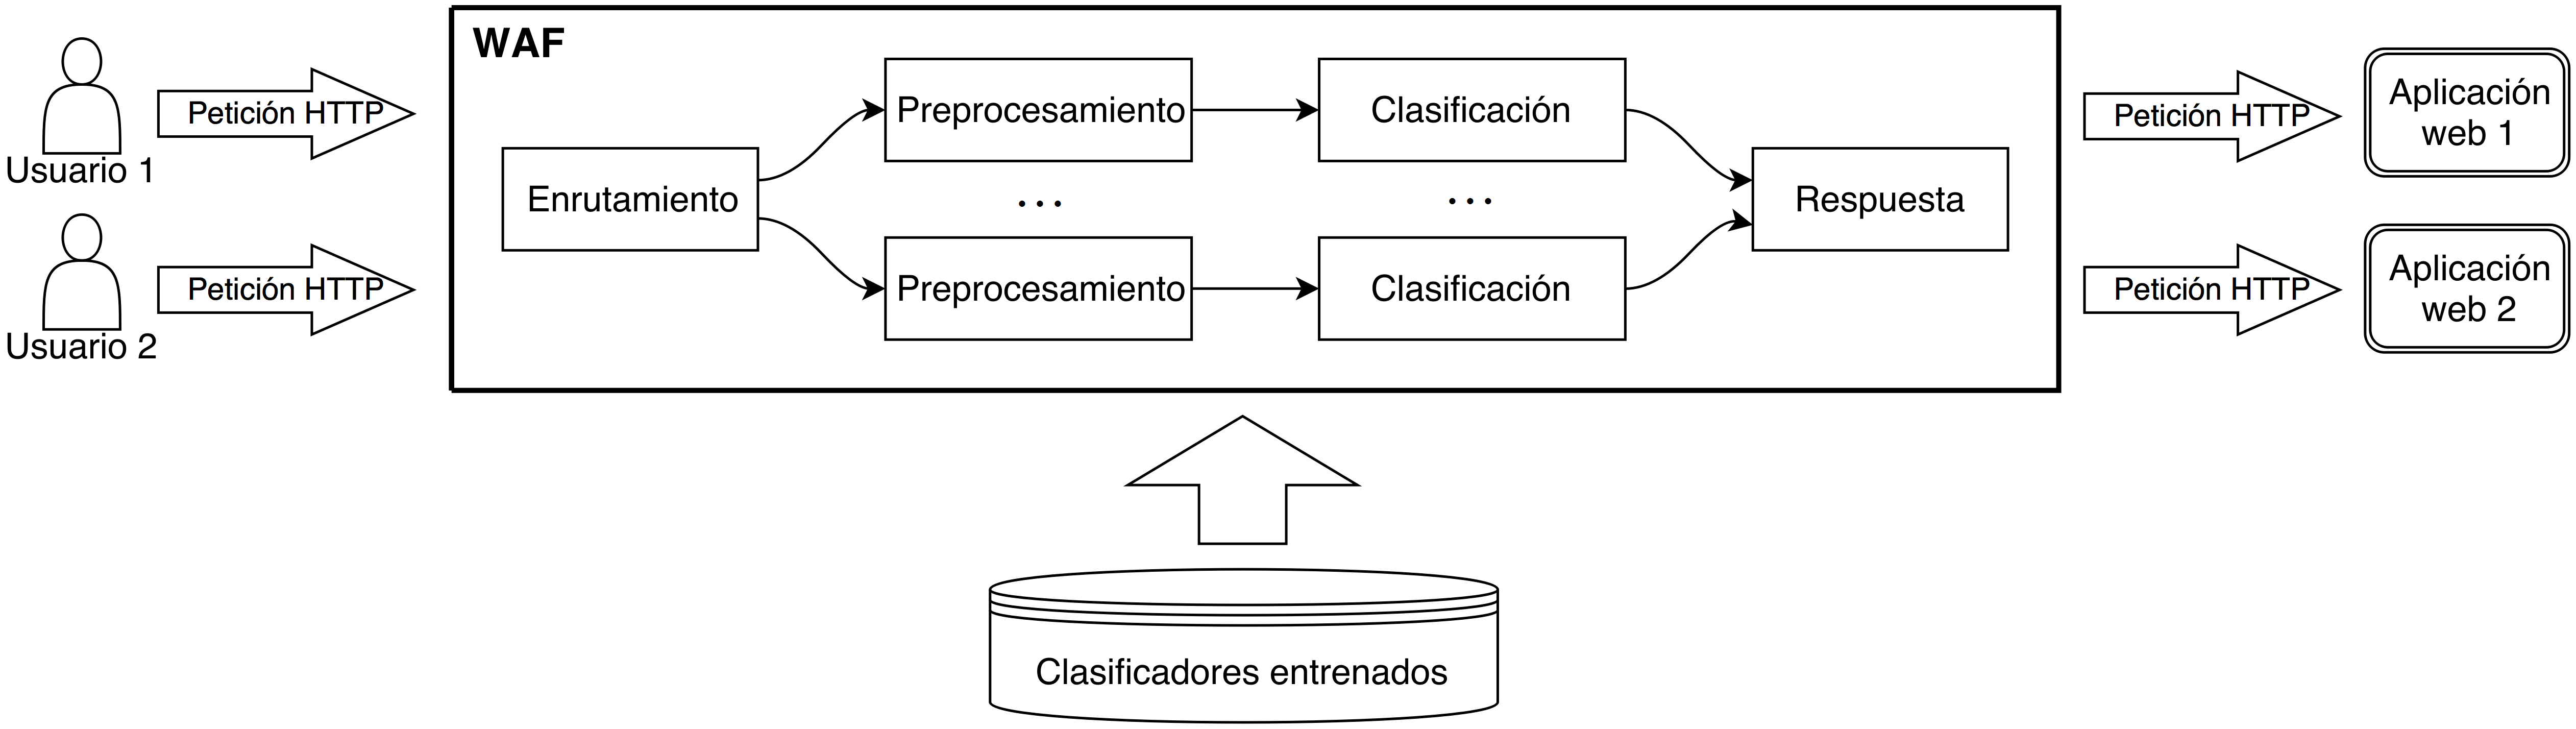
\includegraphics[width=1.1\textwidth]{images/waf-diagram-detection.png}
    \end{center}
\end{frame}

\begin{frame}
    \frametitle{1. Paso de enrutamiento}

    \begin{itemize}[<2->]
        \item
        Identificación del grupo $G_{i}$ de las nuevas peticiones según
        su método HTTP y URL

        \begin{flushleft}
            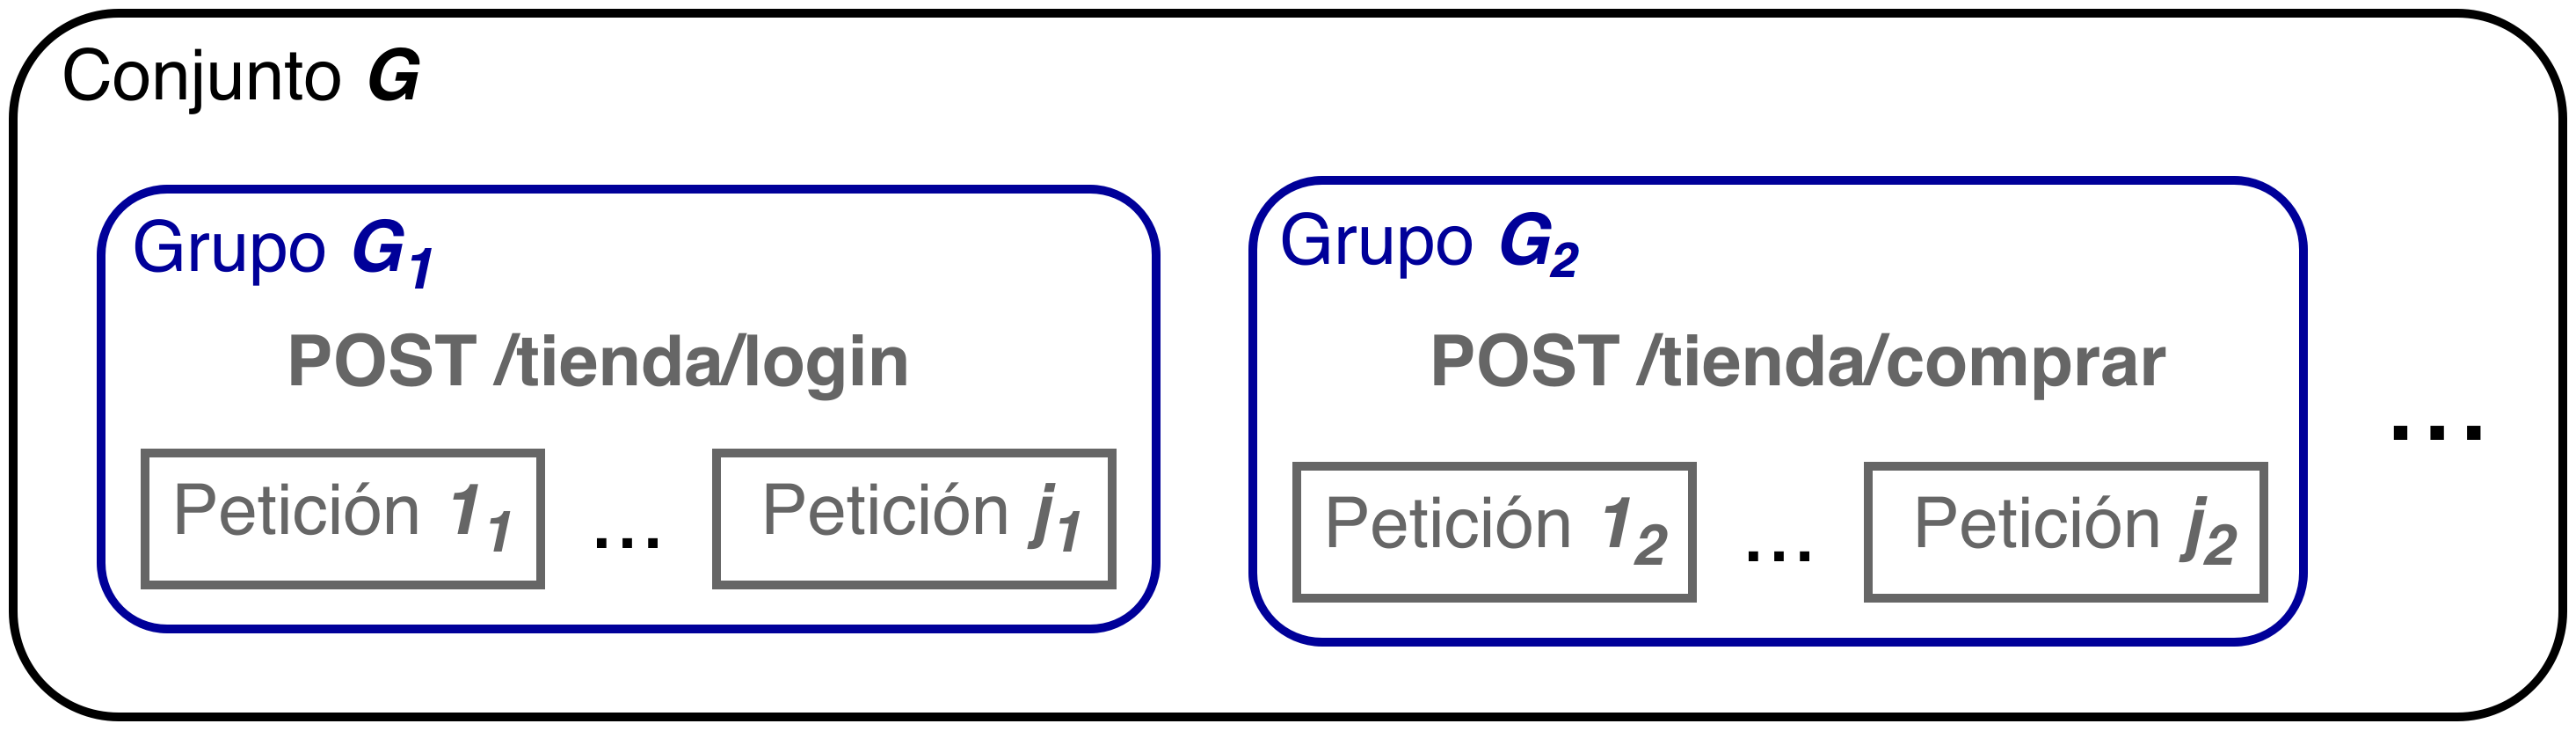
\includegraphics[width=0.9\textwidth]{images/request-groups.png}
        \end{flushleft}

        \item
        Delegación al proceso de extracción de \textit{features} del
        grupo y al clasificador correspondiente
    \end{itemize}
\end{frame}

\begin{frame}
    \frametitle{2. Paso de preprocesamiento}

    \begin{itemize}[<2->]
        \item
        Construcción de vectores de \textit{features} para nuevas peticiones

        \item
        Parámetro de $Q_{i}$ o $B_{i}$ que no aparece en una nueva petición

        \begin{itemize}[<.->]
            \item
            Componentes correspondientes llevan 0
        \end{itemize}

        \item
        Nuevos parámetros que no están en $Q_{i}$ o $B_{i}$

        \begin{itemize}[<.->]
            \item
            No agregan nuevos \textit{features} al vector

            \item
            Están contenidos en la petición completa
        \end{itemize}

        \item
        Vectores nuevos con misma dimensión $n_{i}$ del grupo
    \end{itemize}
\end{frame}

\begin{frame}
    \frametitle{3. Paso de clasificación}

    \begin{columns}
        \column{0.6\textwidth}
        \begin{itemize}[<2->]
            \item
            Uso del hiperplano obtenido para el grupo $G_{i}$

            \item
            Análisis de la posición de nuevas peticiones:

            \begin{itemize}
                \item
                Lado opuesto al origen:

                \begin{itemize}
                    \item
                    Petición normal
                \end{itemize}

                \item
                Mismo lado que el origen:

                \begin{itemize}
                    \item
                    Petición anómala o ataque
                \end{itemize}
            \end{itemize}
        \end{itemize}

        \column{0.4\textwidth}
        \begin{center}
            \uncover<2->{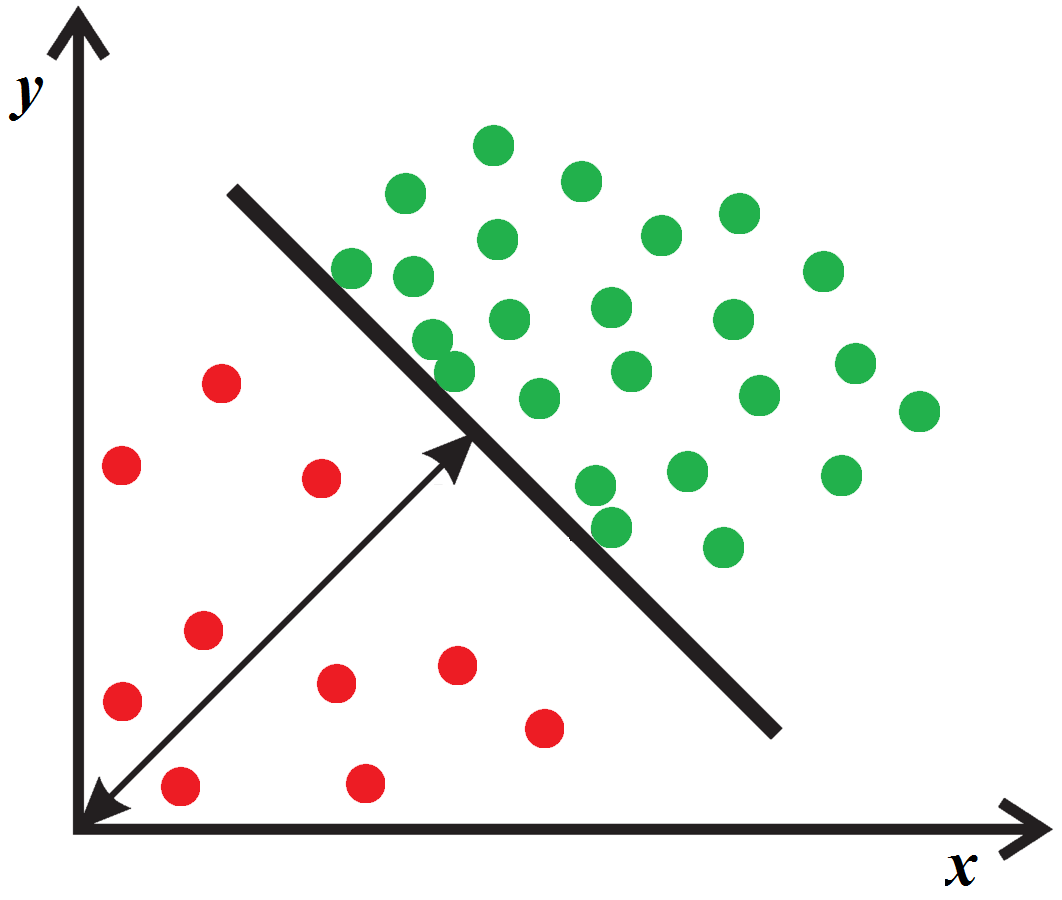
\includegraphics[width=\textwidth]{images/ocsvm-example-2.png}}
        \end{center}
    \end{columns}
\end{frame}

\begin{frame}
    \frametitle{4. Paso de respuesta}

    \begin{itemize}[<2->]
        \item
        Distintas acciones como respuesta al resultado de clasificación

        \item
        Peticiones normales:

        \begin{itemize}
            \item
            Reenvío a las aplicaciones web destino
        \end{itemize}

        \item
        Peticiones anómalas:

        \begin{itemize}
            \item
            Registro en un \textit{log}

            \item
            Opcionalmente: bloqueo de la petición
        \end{itemize}
    \end{itemize}
\end{frame}
